%! TeX root = master.tex
% !TEX program = lualatex

\lecture{10}{28-04-2026}{Deep Learning (Part 2): Convolutional Neural Networks}{}
\subsection{Working with images}
Treating an image as a big vector seems counter-intuitive. An image of a reasonable size yields 
a huge vector (e.g, $x_i \in \mathbb{R}^{536 \cdot 356 \cdot 3} = \mathbb{R}^{572448}$), thus 
a huge amount of parameters in an MLP, but also: 
\begin{itemize}
  \item Small image regions have similar properties and should not be processed independently.
  \item A translation should not affect the results.
\end{itemize}
The goal is therefore to \textbf{reduce the number of parameters and improve robustness}. 
This motivates the use of \textbf{Convolutional Neural Networks (CNNs)}.

\subsection{Convolutional Neural Network (CNN)}
A CNN is a neural network designed to exploit the local structure of its input: nearby elements 
are more related than distant ones (e.g, in an image pixel $(i,j)$ is more related to pixel $(i, j+1)$ than to a more distant one), and the same patterns can appear at different locations. 
This makes CNNs naturally suited for images, but also for any spatially structured signal 
such as audio (1D) or volumetric data (3D).

\subsubsection{2D convolution}
A 2D convolution applies a small filter (kernel) of size $w \times w \times C$ to an input 
of size $W \times W \times C$ by sliding it across all spatial positions (moving horizontally 
and vertically -- hence the term \textbf{2D}, although the operation is internally 3D). At each 
spatial position, the dot product between the kernel and the overlapping $w \times w \times C$ 
region of the input is computed, summing over all channels to produce a single scalar value 
-- measuring how much the local region resembles the filter pattern, regardless of color. 
The resulting 2D array of scalars is called the \textbf{feature map}, of size 
$(W - w + 1) \times (W - w + 1)$. (intuitively the $+1$ is for the first position as if $w = W$ it would result to a $1 \times 1$ feature map)

Formally, the feature map $F$ is defined as:
\[
conv(X, K) = F_{pq} = \sum_{i=1}^{w} \sum_{j=1}^{w} K_{ij} \cdot X_{p+i-1,\, q+j-1}
\]
where $K$ is the kernel and $X$ the input.

E.g, with $X$ of size $3 \times 3 \times 1$ and kernel $K$ of size $2 \times 2 \times 1$, the output is of size $(3-2+1) \times (3-2+1) = 2 \times 2$:
\[
X = \begin{pmatrix} x_{11} & x_{12} & x_{13} \\ x_{21} & x_{22} & x_{23} \\ x_{31} & x_{32} & x_{33} \end{pmatrix}, \quad
K = \begin{pmatrix} k_{11} & k_{12} \\ k_{21} & k_{22} \end{pmatrix}
\]
\[
F = \begin{pmatrix}
k_{11}x_{11} + k_{12}x_{12} + k_{21}x_{21} + k_{22}x_{22} & k_{11}x_{12} + k_{12}x_{13} + k_{21}x_{22} + k_{22}x_{23} \\
k_{11}x_{21} + k_{12}x_{22} + k_{21}x_{31} + k_{22}x_{32} & k_{11}x_{22} + k_{12}x_{23} + k_{21}x_{32} + k_{22}x_{33}
\end{pmatrix}
\]
\subsubsection{Convolutional layer}
A convolutional layer has \textbf{fewer parameters than fully-connected layers} thanks to two 
key properties: 
\begin{itemize}
  \item The parameters of the filter (e.g, $5 \times 5$) are \textbf{learned} (as for the weights of an MLP).
  \item The parameters are \textbf{shared across different spatial locations} (the same filter is applied everywhere).
\end{itemize}

\begin{center}
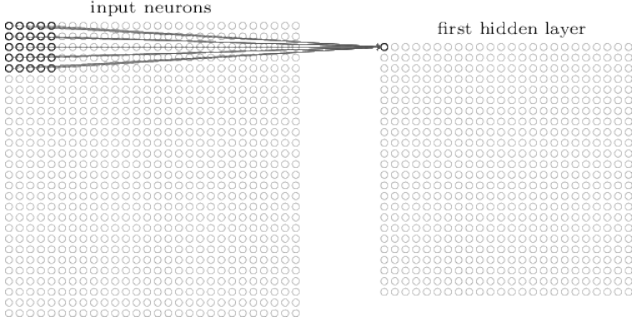
\includegraphics[width=0.4\linewidth]{images/img_20260428_142742.png}
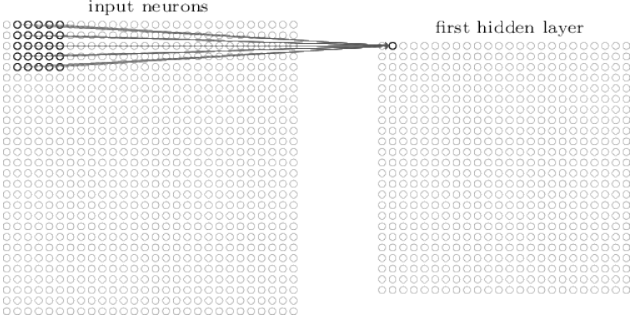
\includegraphics[width=0.4\linewidth]{images/img_20260428_142810.png}
\end{center}

\paragraph{Nonlinearity}
As for MLPs, each convolutional output is passed through an \textbf{activation function} 
(e.g, ReLU). The activation is applied in an \textbf{element-wise} manner, i.e, 
to each spatial location independently.
\begin{center}
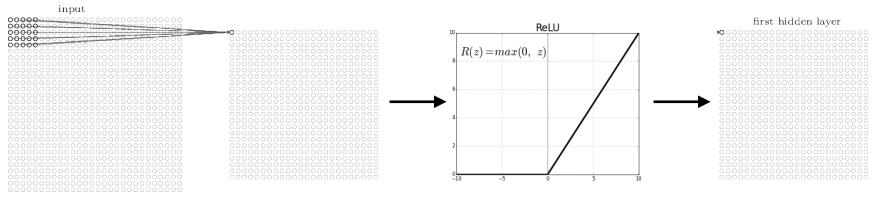
\includegraphics[width=0.8\linewidth]{images/img_20260428_143047.png}
\end{center}

\paragraph{Multiple filters/channels}
We can use multiple filters in a single layer to create multiple \textbf{output channels}. 
Each filter has its own set of learnable parameters. 

\textbf{E.g}, with 3 filters of size $5 \times 5$ on a $28 \times 28$ input, we obtain a 
$3 \times 24 \times 24$ output (3 channels, each of size $24 \times 24$), with 
$3 \cdot 5 \cdot 5 = 75$ learnable parameters.

\begin{center}
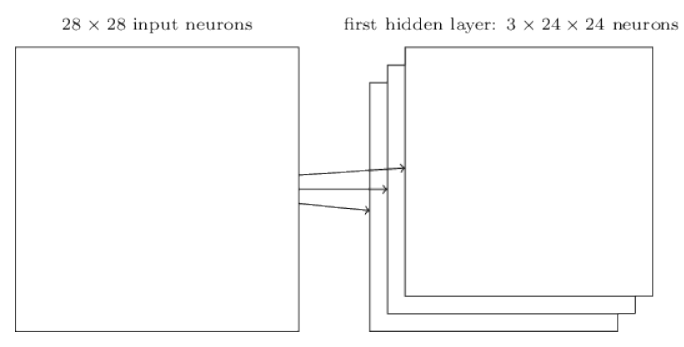
\includegraphics[width=0.5\linewidth]{images/img_20260428_145810.png}
\end{center}

\paragraph{Convolution with multiple input channels}
With multiple input channels (e.g, RGB image with 3 channels), the convolutions are in fact 
done in \textbf{3D}: the kernel has the same number of channels as the input ($w \times h \times C$), 
and the dot product is computed across all channels simultaneously to produce one output value 
per spatial location.

\begin{center}
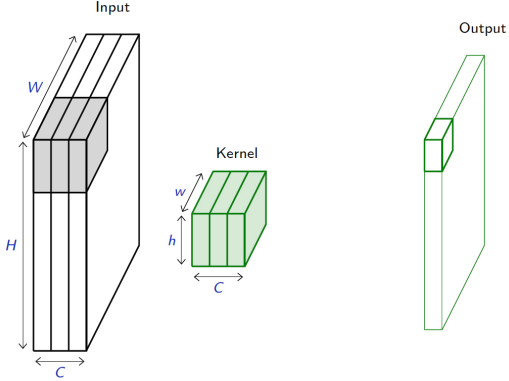
\includegraphics[width=0.4\linewidth]{images/img_20260428_152836.png}
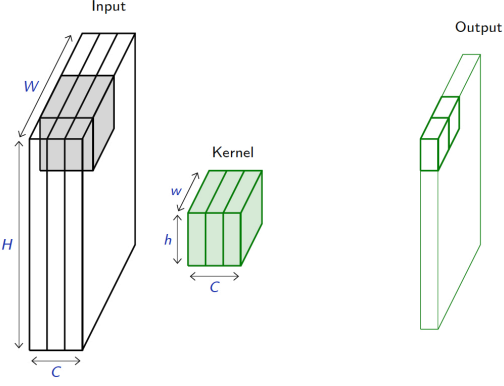
\includegraphics[width=0.4\linewidth]{images/img_20260428_152907.png}
\end{center}

\subsubsection{Pooling layer}
The pooling layer goes from local information to a more \textbf{global representation} by 
aggregating values over a small spatial region. Different pooling strategies exist:
\begin{itemize}
  \item \textbf{Max pooling}: keep the maximum value in each region.
  \item \textbf{Average pooling}: take the average of the values in each region.
\end{itemize}
Pooling reduces the spatial size of the feature maps, which helps reduce the number of 
parameters in subsequent layers and provides some translation invariance.

\begin{center}
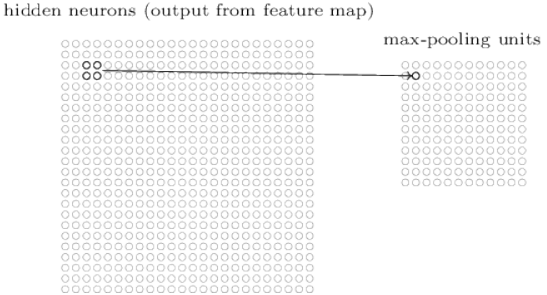
\includegraphics[width=0.5\linewidth]{images/img_20260428_151535.png}
\end{center}

\subsubsection{Padding}
To be able to center the convolution kernel on the boundary locations, \textbf{padding} extends 
the input. This can be done by mirroring or copying the boundary values, or by simply adding zeros 
(zero-padding). With a padding $p = (p_h, p_w)$ it increases the input $(W \times W)$ to $(W + 2 p_h \times W + 2 p_w)$.

E.g, $C \times 3 \times 5$ input with a padding of $(2,1)$ becomes $C \times 7 \times 7$ (2 lines of zeroes (zero-padding) up and down, and 1 column of zeroes to the left and to the right). 
\begin{center}
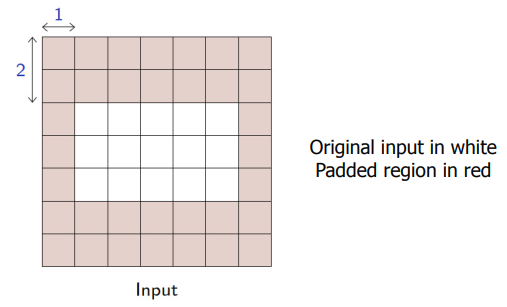
\includegraphics[width=0.4\linewidth]{images/img_20260428_153607.png}
\end{center}

\subsubsection{Convolution stride}
In a standard convolution, the filter is shifted pixel by pixel. The shifts can be made larger 
by increasing the \textbf{stride} $s = (s_h, s_w)$: the filter jumps $s_h$ pixels in height 
and $s_w$ pixels in width at each step, reducing the output size to 
$\left\lfloor\frac{W}{s_h}\right\rfloor \times \left\lfloor\frac{W}{s_w}\right\rfloor$.

E.g, stride of $(2,2)$ on a padded input with a $3 \times 3$ kernel: the kernel only 
hops every 2 pixels, producing a smaller output.

\begin{center}
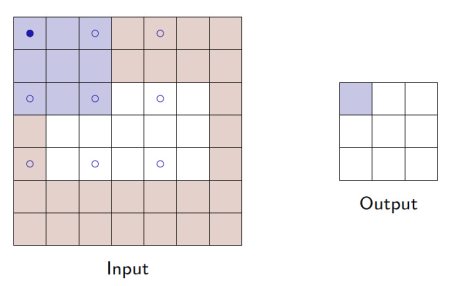
\includegraphics[width=0.33\linewidth]{images/img_20260428_153939.png}
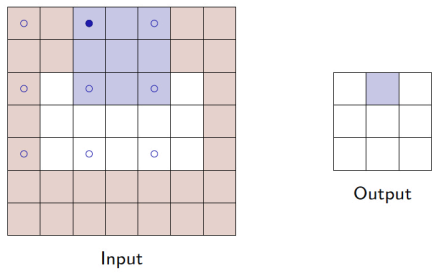
\includegraphics[width=0.32\linewidth]{images/img_20260428_154032.png}
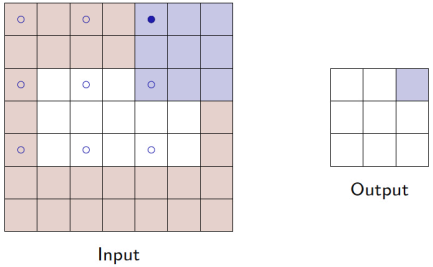
\includegraphics[width=0.32\linewidth]{images/img_20260428_154053.png}
\end{center}

\textbf{Goal of strided convolution}: Reduce the spatial size of the feature map (downsampling), 
which decreases the computational cost and memory usage. 

\textbf{Drawback}: Loss of spatial information (skipping pixels) which may hurt the model 
if fine-grained details are important.

\subsubsection{CNN architecture}
We can stack convolution + activation + pooling operations to build a CNN. 
\begin{itemize}
  \item The number of channels can vary between layers (e.g, first 3, then 6, then 16, $\ldots$).
  \item The size of the filters can vary (e.g, first $5 \times 5$, then $3 \times 3$).
\end{itemize}

\begin{center}
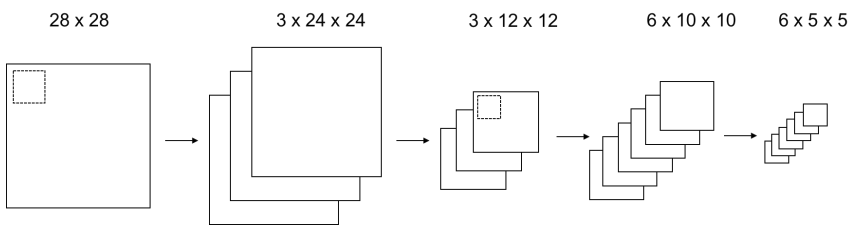
\includegraphics[width=0.8\linewidth]{images/img_20260428_153312.png}
\end{center}

\paragraph{Output layer for vector predictions}
Eventually, one typically wants to output a vector, e.g.,
\begin{itemize}
  \item A vector of class probabilities for classification.
  \item A vector of 3D joint coordinates for human pose estimation.
\end{itemize}
This can be achieved by appending \textbf{fully-connected (FC) layers} at the end of the CNN. 
This requires \textbf{vectorizing} the last convolutional output first 
(e.g, $3 \times 12 \times 12 \to 432$-dimensional vector).

\begin{center}

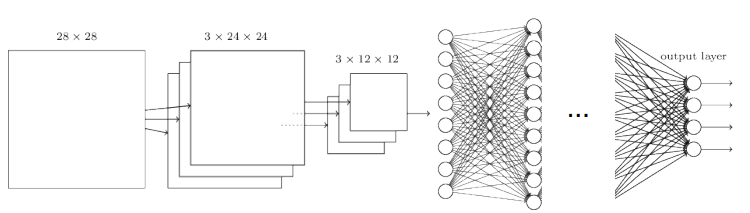
\includegraphics[width=0.8\linewidth]{images/img_20260428_154550.png}
\end{center}

\subsubsection{Normalization layers}
Inspired by the fact that data normalization can help, several layers have been developed to 
normalize the feature maps inside the network. They differ by the dimensions over which the 
mean and variance are computed:
\begin{itemize}
  \item \textbf{Batch normalization} (Ioffe \& Szegedy, ICML 2015): normalizes across the batch (per channel).
  \item \textbf{Layer normalization} (Ba et al., 2016): normalizes across all channels (per sample).
  \item \textbf{Instance normalization} (Ulyanov et al., 2016): normalizes per channel and per sample.
  \item \textbf{Group normalization} (Wu \& He, 2018): normalizes within groups of channels.
\end{itemize}
Notation: $N$ = number of samples in a mini-batch, $C$ = number of channels, $(H, W)$ = size of the feature map.

\begin{center}
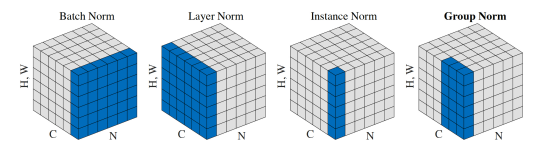
\includegraphics[width=0.8\linewidth]{images/img_20260428_154830.png}
\end{center}

\subsubsection{CNN: Learning}
Learning the weights of CNN layers is done in the same manner as for MLPs, using 
\textbf{stochastic gradient descent (SGD)} with mini-batches. The same idea of 
\textbf{backpropagation} is applicable to convolutional layers.

\textbf{Gradient of pooling layers} depends on the strategy:
\begin{itemize}
  \item \textbf{Average pooling}: the gradient is backpropagated to all neurons used during pooling.
  \item \textbf{Max pooling}: the gradient is backpropagated only to the neuron that corresponded to the maximum value (the others get zero).
\end{itemize}

The same SGD extensions apply (Momentum, Adaptive learning rates like ADAM), as well as the same 
regularization techniques (Early stopping, Weight decay, Dropout).

\subsubsection{CNN: Interpretation}
A CNN can be thought of as \textbf{jointly learning the data representation and the classifier} 
(or regressor): the early layers learn low-level features (edges, textures), the middle layers 
learn parts (eyes, wheels), and the deeper layers learn high-level concepts (faces, objects).

\begin{center}
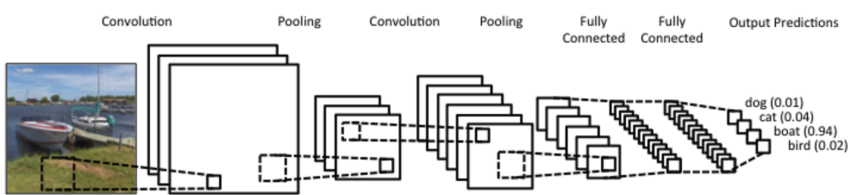
\includegraphics[width=0.8\linewidth]{images/img_20260428_155310.png}
\end{center}

One can visualize the features extracted at different layers (Zeiler \& Fergus, ECCV 2014):
\begin{itemize}
  \item \textbf{Layer 1}: oriented edges, color blobs.
  \item \textbf{Layer 2}: textures, simple patterns (circles, stripes).
  \item \textbf{Layer 3}: more complex patterns, parts of objects (faces, wheels, text).
\end{itemize}

\subsection{Semantic segmentation}
When working with images, one does not necessarily want to simply classify them. 
\textbf{Semantic segmentation} is the task of assigning a label to \textbf{every pixel} 
in the input image (e.g, sky, road, bridge, fence, $\ldots$).
\begin{center} 
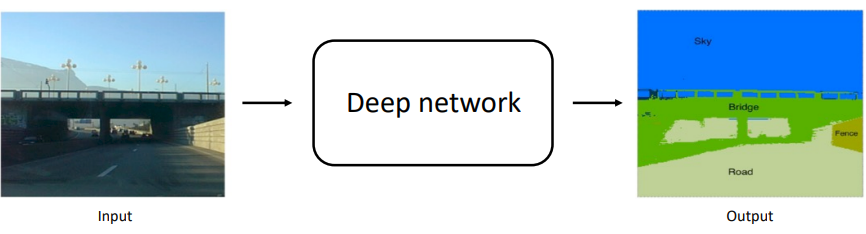
\includegraphics[width=0.75\linewidth]{images/img_20260428_160039.png}
\end{center}


\subsubsection{Problem with standard CNNs}
With convolutions (without padding and/or with stride $>1$) and pooling layers, the size of the 
feature maps \textbf{decreases} at every layer. With the operations seen so far, we have no way 
of \textbf{increasing} this size back to the original resolution, which is needed for pixel-wise 
prediction.

\subsubsection{Solutions}
Two main solutions to upsample the feature maps:
\begin{itemize}
  \item \textbf{Upsampling}, followed by convolutions (e.g, nearest-neighbor or bilinear upsampling, then convolution to refine).
  \item \textbf{Transposed convolutions} (also known as deconvolutions or fractionally-strided convolutions).
\end{itemize}

\subsubsection{1D convolution as a matrix product}
Before looking at transposed convolutions, let us first observe that a 1D convolution can be 
expressed as a \textbf{matrix product}. The input is a vector of dimension $W$, the kernel of 
size $w$, and the output of dimension $W - w + 1$.

\textbf{Example} : with input $[1,4,-1,0,2,-2,1,3,3,1]$ and kernel $[1,2,0,-1]$:
\[
z = \begin{pmatrix} 9 \\ 0 \\ 1 \\ 3 \\ -5 \\ -3 \\ 6 \end{pmatrix}
=
\begin{pmatrix}
1 & 2 & 0 & -1 & 0 & 0 & 0 & 0 & 0 & 0 \\
0 & 1 & 2 & 0 & -1 & 0 & 0 & 0 & 0 & 0 \\
& & & \ddots & & & & & & \\
0 & 0 & 0 & 0 & 0 & 0 & 1 & 2 & 0 & -1
\end{pmatrix}
\begin{pmatrix} 1 \\ 4 \\ -1 \\ 0 \\ 2 \\ -2 \\ 1 \\ 3 \\ 3 \\ 1 \end{pmatrix}
\]

So a convolution can be represented by a \textbf{rectangular matrix} going from dimension $W$ 
to dimension $W - w + 1$.

\subsubsection{Transposed convolution}
Since a convolution can be represented by a rectangular matrix going from dimension $W$ to 
dimension $W - w + 1$, \textbf{increasing the dimensionality} can be achieved by using the 
\textbf{transposed matrix}:
\[
\begin{pmatrix}
w_1 & w_2 & w_3 & 0 & 0 & 0 \\
0 & w_1 & w_2 & w_3 & 0 & 0 \\
0 & 0 & w_1 & w_2 & w_3 & 0 \\
0 & 0 & 0 & w_1 & w_2 & w_3
\end{pmatrix}^T 
=
\begin{pmatrix}
w_1 & 0 & 0 & 0 \\
w_2 & w_1 & 0 & 0 \\
w_3 & w_2 & w_1 & 0 \\
0 & w_3 & w_2 & w_1 \\
0 & 0 & w_3 & w_2 \\
0 & 0 & 0 & w_3
\end{pmatrix}
\]
This goes from dimension $W - w + 1$ to dimension $W$, so it \textbf{upsamples} the input 
(transposed conv is also called \emph{up-convolution}).

\paragraph{Example of 1D transposed convolution}
With input $[2, 3, 0, -1]$ ($W = 4$) and kernel $[1, 2, -1]$ ($w = 3$): each input value 
multiplies the entire kernel, and the resulting scaled kernels are summed at shifted positions:
\begin{itemize}
  \item Input value 2 : $[2, 4, -2]$ at position 0.
  \item Input value 3 : $\to [3, 6, -3]$ at position 1.
  \item Input value 0 : $\to \to [0, 0, 0]$ at position 2.
  \item Input value -1: $\to \to \to [-1, -2, 1]$ at position 3.
\end{itemize}
Summing them gives the output $[2, 7, 4, -4, -2, 1]$ of dimension $W + w - 1 = 6$.

So it goes from dimension $W$ to dimension $W + w - 1$

In matrix form \[
  \begin{pmatrix}
    1 & 2 & -1 & 0 & 0 & 0 \\
    0 & 1 & 2 & -1 & 0 & 0 \\
    0 & 0 & 1 & 2 & -1 & 0 \\
    0 & 0  & 0 & 1 & 2 & -1
\end{pmatrix} ^T 
  \begin{pmatrix}
    2 \\
    3 \\
    0 \\
    -1
\end{pmatrix}
= 
\begin{pmatrix}
  2 \\
  7 \\
  4 \\
  -4 \\
  -2 \\
  1
\end{pmatrix}
\]

\subsubsection{2D convolution as matrix product}
A similar matrix representation can be obtained for 2D convolutions:
\begin{itemize}
  \item The input is \textbf{vectorized}, e.g, by concatenating its columns (e.g, matrix $4 \times 3$ to a matrix $12 \times 1$).
  \item The matrix is obtained by spreading the different columns of the kernel at the matching locations.
\end{itemize}
The same trick (using the transpose) gives 2D transposed convolutions for upsampling.

\subsubsection{Fully-convolutional networks}
Stacking upsampling-convolutions, or transposed convolutions, after regular ones lets us go 
back to the original spatial resolution. This is the principle of \textbf{fully-convolutional 
networks (FCNs)} like \textbf{U-Net} (Ronneberger et al., MICCAI 2015), widely used for 
semantic segmentation. 

The U-Net architecture has a characteristic ``U'' shape:
\begin{itemize}
  \item A \textbf{contracting path} (encoder): regular convolutions + pooling reduce the spatial size while increasing the number of channels.
  \item An \textbf{expanding path} (decoder): transposed convolutions (up-conv) increase the spatial size back to the original resolution while decreasing the number of channels.
  \item \textbf{Skip connections} between matching encoder and decoder levels (copy and crop) allow the decoder to recover spatial details lost during downsampling.
\end{itemize}

\begin{center}
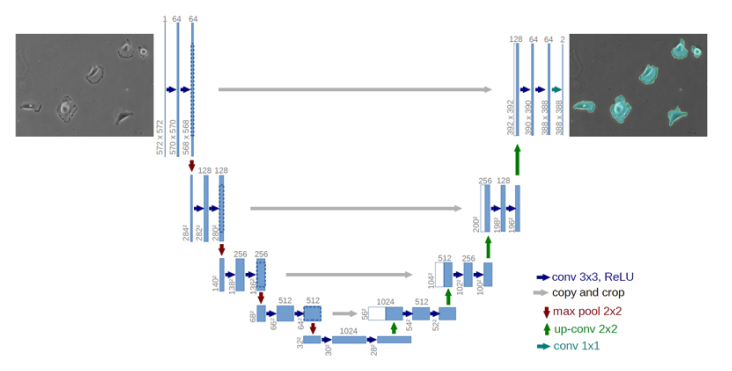
\includegraphics[width=0.6\linewidth]{images/img_20260428_161220.png}
\end{center}

\subsection{The keys to the success of Deep Learning}
\begin{itemize}
  \item \textbf{Big data}: large annotated datasets, e.g, ImageNet (Russakovsky et al., 2015) with millions of labeled images.
  \item \textbf{GPUs}: massively parallel computations make training of deep networks feasible.
\end{itemize}

\subsubsection{Tricks of the trade}
\begin{itemize}
  \item \textbf{Pre-training}: people often start with a standard architecture (e.g, ResNet) pre-trained on ImageNet, then fine-tune (adapt) it on the target task. This transfers learned features and accelerates training.
  \item \textbf{Data augmentation}: artificially increase the dataset size by applying transformations that preserve the label, e.g, for images: flip, rotate, affine transform, color jittering, $\ldots$
  \item \textbf{Learning rate scheduling}: 
    \begin{itemize}
      \item Decrease the learning rate $\eta$ after a pre-defined number of epochs (step-decay (divide $\eta $ by a fix factor after a number of predefined epochs)).
      \item Use a cyclic learning rate (make $\eta$ oscillates between a min and max value).
    \end{itemize}
\end{itemize}
\begin{center}
   
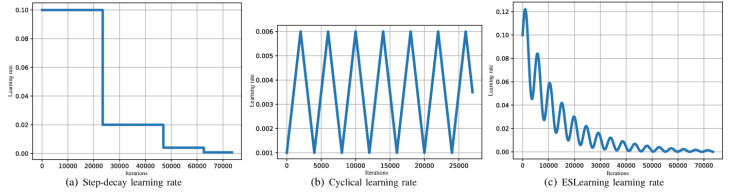
\includegraphics[width=0.8\linewidth]{images/img_20260428_161951.png}
\end{center}

\subsection{Despite the success: Adversarial examples}
Even very accurate deep networks can be fooled by \textbf{adversarial examples}: small, 
imperceptible perturbations $\Delta I$ added to the input image $I$ can completely change the 
prediction. 

\paragraph{Example}

An image classified as ``Giant Panda'' with 99.32\% confidence, after adding a 
tiny perturbation ($+0.03$), is classified as ``Shark'' with 93.89\% confidence (or as 
``Goldfish'' with 95.15\% confidence with a different perturbation), even though the modified 
image still looks like a panda to humans.

\begin{center}
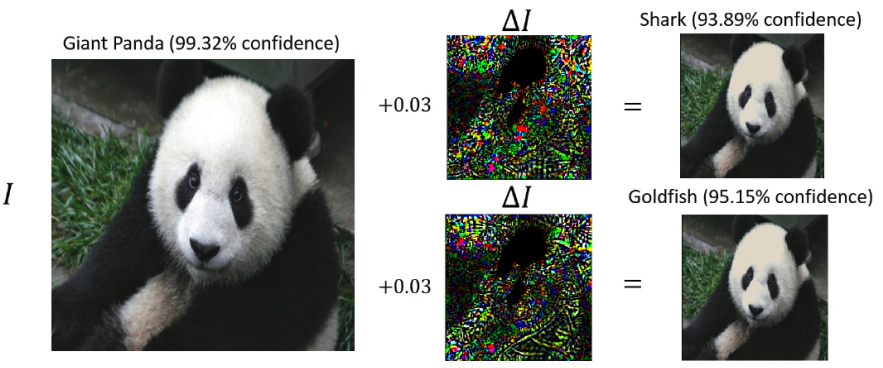
\includegraphics[width=0.7\linewidth]{images/img_20260428_162246.png}
\end{center}

\textbf{Intuition}: Deep networks learn highly non-linear decision boundaries in a 
high-dimensional input space. Even if the perturbation is small in pixel space, it can move 
the input across a decision boundary in the network's internal feature space. Networks rely on 
specific patterns/textures rather than the high-level semantic concepts humans use, so 
carefully crafted perturbations targeting these patterns can fool the network without changing 
the human-perceived content of the image.

This shows that despite their success, deep networks are not as robust as humans, and 
robustness to adversarial examples remains an active area of research.

\clearpage
